\definecolor{tiffanyblue}{RGB}{129,216,208}
\definecolor{bangdiblue}{RGB}{0,149,182}
\definecolor{kleinblue}{RGB}{0,47,167}
\definecolor{kabuliblue}{RGB}{26,85,153}
\definecolor{purple}{RGB}{138,43,226}
\usepgfplotslibrary{groupplots}
\begin{figure}[t!]
  \centering
  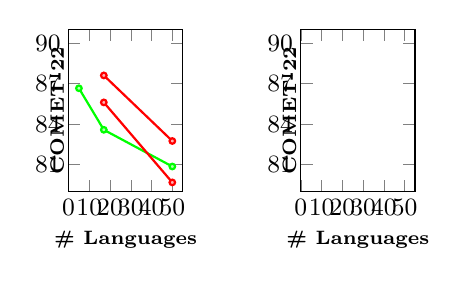
\begin{tikzpicture}
    \pgfplotsset{set layers}
    % \scriptsize{
    % % 全局图例单独绘制
    % \begin{axis}[
    % at={(2,1)},
    % width=0.45\textwidth,
    %   height=0.2\textwidth,
    %   hide axis,
    %   xmin=0, xmax=0.5, ymin=0, ymax=0.5,
    %   legend style={
    %     draw=none,
    %     fill=none,
    %     font=\small,
    %     column sep=0.3cm,
    %     at={(0.67,1.9)},
    %     anchor=north
    %   },
    %   legend columns=1
    % ]
    %   \addlegendimage{red, mark=diamond*, mark size=1.5pt, thick, mark options={solid, fill=red}}
    %   \addlegendentry{Sample Ratio - 0.1}
    %   \addlegendimage{blue, mark=triangle*, mark size=1.5pt, thick, mark options={solid, fill=blue}}
    %   \addlegendentry{Sample Ratio - 0.5}
    %   \addlegendimage{green!30, mark=square*, mark size=1.5pt, thick, mark options={solid, fill=green!30}}
    %   \addlegendentry{Sample Ratio - 1.0}
    % \end{axis}
    % }
    \scriptsize{
    \begin{groupplot}[
      group style={group size=2 by 1, horizontal sep=1.5cm, vertical sep=1cm},
      % xmajorgrids,
      % grid style={dashed, gray!50},
      width=0.25\textwidth,
      height=0.3\textwidth,
      xlabel={\# Languages},
      ylabel={COMET-22},
      xlabel style={font=\bfseries, yshift=0em},
      ylabel style={font=\bfseries, yshift=-2em},
      yticklabel style={font=\small},
      xticklabel style={font=\small},
      title style={font=\bfseries},
      xmin=0, xmax=55, 
      xtick={0, 10, 20, 30, 40, 50},
    ]
    % % 第一行:Model 1
    % \nextgroupplot[title={\{De, Zh, Cs, Ru\}$\leftrightarrow$En}, ymin=84, ymax=91, ytick={82, 84, 86,88}]
    % % \addplot[red, mark=diamond*, mark size=1.5pt, thick, mark options={solid, fill=red}] 
    % %   coordinates {(5, 87.64) (9, 86.76) (17, 84) (50, 82.37)};

    % % \addplot[blue, mark=triangle*, mark size=1.5pt, thick, mark options={solid, fill=blue}] 
    % %   coordinates {(5, 87.98) (17, 86.15) (50, 83.54)};

    % \addplot[green, mark=square*, mark size=1.5pt, thick, mark options={solid, fill=green!30}] 
    %   coordinates {(5, 87.87) (17, 86.27) (50, 84.88)};
      
    \nextgroupplot[title={}, ymin=79, ymax=91, ytick={81, 84, 87, 90}]
    % \addplot[red, mark=diamond*, mark size=1.5pt, thick, mark options={solid, fill=red}] 
    %   coordinates {(5, 86.76) (9, 84.97) (17, 79.76) (50, 76.37)};
    % \addplot[red, mark=diamond*, mark size=1.5pt, thick, mark options={solid, fill=red}] 
    %   coordinates {(5, 86.76) (17, 79.76) (50, 76.37)};

    % \node[anchor=south, fill=white, rounded corners=2pt, inner sep=1pt] at (axis cs:18,86.76) {\scriptsize $86.76/86.72/86.65$};
    % \node[anchor=north, fill=white, rounded corners=2pt, inner sep=1pt] at (axis cs:50,76.37) {\scriptsize $76.37$};
    % \draw[<->, gray, thick] (axis cs:5,86.76) -- (axis cs:5,76.37) 
    %   node[midway, above, font=\small, text=gray, xshift=1.5em, yshift=-4em] {\scriptsize{$\Delta = 10.39$}};
    % \draw[ dotted, gray] (axis cs:5,76.37) -- (axis cs:50,76.37) ;
      
    % \addplot[blue, mark=triangle*, mark size=1.5pt, thick, mark options={solid, fill=blue}] 
    %   coordinates {(5,86.72) (17, 83.16) (50, 78.06)};
    \addplot[green, mark=*, mark size=1.0pt, thick, mark options={solid, fill=green!30}] 
      coordinates { (5, 86.65) (17, 83.57) (50, 80.85)};
    % Sample Ratio 0.1
    % \addplot[red, mark=square*, mark size=1.5pt, thick, mark options={solid, fill=red!30}] 
    %   coordinates { (5, 86.65) (17, 87.60) (50, 86.65)};

    \addplot[red, mark=*, mark size=1pt, thick, mark options={solid, fill=red!30}] 
      coordinates {  (17, 87.60) (50, 82.74)};

    \addplot[red, mark=*, mark size=1pt, thick, mark options={solid, fill=red!30}] 
      coordinates {  (17, 85.60) (50, 79.67)};

    \nextgroupplot[title={}, ymin=79, ymax=91, ytick={81, 84, 87, 90}]
    % \node[anchor=north, fill=white, rounded corners=2pt, inner sep=1pt] at (axis cs:50,80.85) {\scriptsize $80.86$};
    % \draw[<->, gray] (axis cs:50,86.65) -- (axis cs:50,80.85) 
    %   node[midway, above, font=\small, text=gray, xshift=-2.5em, yshift=0em] {\scriptsize{$\Delta = 5.79$}};
    % \draw[ dotted, gray, thick] (axis cs:5,86.65) -- (axis cs:50,86.65) ;
    
    % \nextgroupplot[title={En→\{De, Zh, Cs, Ru\}}, ymin=75, ymax=90, ytick={75, 80, 85, 90}]
    % \addplot[red, mark=diamond*, mark size=1.5pt, thick, mark options={solid, fill=red}] 
    %   coordinates {(5, 88.52) (9, 88.55) (17, 88.24) (50, 88.37)};

    % \addplot[blue, mark=triangle*, mark size=1.5pt, thick, mark options={solid, fill=blue}] 
    %   coordinates {(5,89.23) (17, 89.13) (50, 89.02)};
    % \addplot[green!30, mark=square*, mark size=1.5pt, thick, mark options={solid, fill=green!30}] 
    %   coordinates {(5, 89.08) (17, 88.96)  (50, 88.91)};
    % % 第二行:Model 2
    % \nextgroupplot[ymin=75, ymax=90, ytick={75, 80, 85, 90}]
    % \addplot[blue, mark=triangle*, mark size=1.5pt, thick, mark options={solid, fill=blue}] 
    %   coordinates {(5,86.72) (17, 83.16) (50, 78.06)};
    % \nextgroupplot[ymin=84, ymax=90, ytick={84, 86, 88, 90}]
    % \addplot[blue, mark=triangle*, mark size=1.5pt, thick, mark options={solid, fill=blue}] 
    %   coordinates {(5,89.23) (17, 89.13) (50, 89.02)};
    
    % \nextgroupplot[ymin=82, ymax=90, ytick={82, 84, 86, 88, 90}]
    % \addplot[blue, mark=triangle*, mark size=1.5pt, thick, mark options={solid, fill=blue}] 
    %   coordinates {(5, 87.98) (17, 86.15) (50, 83.54)};
      


    % % 第三行:Model 3
    % \nextgroupplot[ymin=75, ymax=90, ytick={75, 80, 85, 90}]
    % \addplot[green, mark=square*, mark size=1.5pt, thick, mark options={solid, fill=green}] 
    %   coordinates { (5, 86.65) (17, 83.57) (50, 80.85)};
    % % \node at (0.5,-10.25) {(c) XX-En};
    % \nextgroupplot[ymin=84, ymax=90, ytick={84, 86, 88, 90}]
    % \addplot[green, mark=square*, mark size=1.5pt, thick, mark options={solid, fill=green}] 
    %   coordinates {(5, 89.08) (17, 88.96)  (50, 88.91)};
    
    % \nextgroupplot[ymin=83, ymax=89, ytick={84, 86, 88}]
    % \addplot[green, mark=square*, mark size=1.5pt, thick, mark options={solid, fill=green}] 
    %   coordinates {(5, 87.87) (17, 86.27) (50, 84.88)};

    \end{groupplot}
    }
  \end{tikzpicture}
  \vskip 0.1in
  \caption{Performance }
  \label{fig:}
\end{figure}